\documentclass{article}
\usepackage{graphicx} % Required for inserting images
\usepackage{float}

\title{Modélisation}
\author{Peng Cédric, Lin Michel}
\date{\today}

\begin{document}

\maketitle

\section{Présentation}
Nous avons décidé de faire un système de réservation d'entré et de billet pour un festival
de restaurants séparé en plusieurs zones où les utilisateurs doivent passer par une préinscription
pour participer au festivals pour une période précise, puis d'une sélection et achat de leur billet
d'entré avec créneaux d'achat.\\
De nouvelle sélection sera faite apres la fin d'une selection si il reste des places dans le festival et que le festival n'a pas encore démarré. \\
L'utilisateur devra payer le prix du billet qui dépend de plusieurs
facteurs(zone, statut, pass, ...) et acheter des "crédits" qui feront office de monnaie dans les restaurants. 
Un utilisateur ne peut avoir qu'un seul billet par période de festival.
\\
\\
Une fois dans le festival, le billet fera office de carte où
sera stocké les crédits acheté précédemment. Le billet sera alors nécessaire 
pour consommer ce qui permettra ainsi de conserver un historique des consommation et activité fait par un utilisateur. 
\\
\\
Nos restaurants possèdent chacun un menu avec des plats et des prix selon la zone où elle se situe. La zone 1 correspond au restaurant
dont les prix des plats ne dépasse pas 50 crédits, la zone 2 au restaurants avec des prix
ne dépassant pas 200 crédits, et enfin la zone 3 ou les restaurants seront qualifié de gastronomique avec des prix pouvant aller au delà de 200 crédits.
Il sera possible de consulter l'addition détaillé de chaque consommation dans un restaurants avec les plats, les quantités prise et la note total.


\section{Modèle E\textbackslash R}

\subsection{Réservation}
\begin{itemize}
    \item Une phase de préinscription pour pouvoir être sélectionné par la suite.\\
    \item \textbf{Check : on peut participer a la préselection que 2 semaine avant le début du festival}
    \item Une phase de sélection qui permet de choisir les utilisateurs qui seront choisit pour l'achat du billet.\\
    \textbf{Trigger : Un utilisateur ne peut pas faire la sélection si il n'a pas fait la préinscription}\\
    \textbf{trigger : Les selections et les préinscriptions se déroule que pendant l'intervalle de temps autorisé}
    $Selection(id\_u,id\_festival) \subset Preinscription(id\_u,id\_festival)$
    \item Une fois sélectionné l'utilisateur aura une journée précis pour acheter son billet.\\
    \textbf{Trigger :  L'achat d'un billet ne peut se faire que si l'utilisateur à fait la préinscription, passé la sélection et durant la journée fixé.}\\
    $Utilisateur\_Billet(id\_u,id\_festival) \subset Selection(id\_u,id\_festival)$ \\$CURRENT\_TIME \in Selection(creneau)$

    \item Si des places sont encore disponible on peut relancer une phase de sélection jusqu'a qu'il n'en reste plus ou que le festival commence.
    \item Les personnes qui ont été sélectionnées et qui n'ont pas procédé à un achat peuvent à nouveau l'être.\\
    \textbf{Trigger :  La sélection est faite avec les personnes qui se sont préinscrite mais qui n'avait pas été sélectionné ou fait d'achat}
    \item Un tarif selon le statut de l'utilisateur (retraité,etc..)\\
    \textbf{Fonction : Vérifier le status de l'utilisateur lors de l'achat}
    \item Possibilité d'acheter un pass pour avoir des avantages.
    \item Un tarif selon les zones d'accès prise. Un billet ne donne par défaut pas accès à toute les zones du festival. 
    L'utilisateur doit préciser à quelle zone il souhaite avoir accès. Un coût supplémentaire sera ajouté selon les zones choisies.\\
    \textbf{Fonction : Le prix du ticket d'entré correspond à la somme des différents tarifs (statut,période, bonus pass,...)}
    
    \item Un système de points de fidélité en fonction du nombre de crédit acheté
    \textbf{Trigger : Les points de fidélité sont réinitialisés si l'utilisateur n'est pas venu depuis plus d'un an}
    \item Possibilité de tracer tout les achats effectués par un utilisateur 
   
    \item Le nombre de billet disponible pour une période est défini a l'avance 
    
    \item La phase de sélection continue jusqu'à la date de début du festival.\\
    \textbf{Trigger : Il doit resté des places disponibles }
    \item  \textbf{Contrainte d'unicité : On ne peut acheter que un seul billet pour une période donnée }
    \item \textbf{Trigger : On ne peut pas acheter de billet si le festival a déjà commencé.}
\end{itemize}
\subsection{Pass}
\begin{itemize}
    \item Plusieurs sorte de nom/type de bonus (cuillère de bronze, couteau de fer, fourchette d'or) qui chacun offre différentes réduction sur le prix du billet d'entré ainsi qu'un bonus de crédit inital .
    \item \textbf{Fonction : Un utilisateur ne peut pas avoir plusieurs pass actif, seul celui avec la date d'achat la plus récente est pris en compte} 
    \item Un prix selon le type et de la durée du pass \\
    \textbf{Check : Date = 1mois | 6mois | 1an}
    \item Ajout d'un bonus de crédit initial si l'utilisateur possède un pass 
    \textbf{Trigger : Le crédit initial dépend du pass }
    \item réduction du prix du billet d'entré selon le type de pass
    \textbf{Trigger : Suivant le pass que l'utilisateur possede}
    \item un pass est composé d'une durée et d'un nom/type de bonus. 
    \item le nom/type du bonus détermine la réduction et le bonus de crédit initial
    \item plusieurs utilisateurs peut avoir le meme type de pass 
\end{itemize}

\subsection{Restaurant}
\begin{itemize}
    \item Les restaurants seront chacun situé dans une zone qui détermine leur type (chère, moyen, très chère) \\
    \textbf{Contrainte d'unicité  : Un restaurant ne peut pas etre dans plusieurs zones en meme temps}
    \textbf{Trigger : Le billet de l'utilisateur doit donner accès a la zone du restaurant pour y consommer}
    \item Les restaurants possèdent un menu avec différents plats et prix \\
    \textbf{Contrainte d'unicité  : Il ne peut pas avoir le meme plat avec un prix different}
    \item Chaque plat ne peut être vendu qu'un nombre limité de fois par jour\\
    \textbf{Trigger : On ne peut pas commandé le plat en question s'il n'est plus en stock}
    \item On ne peut pas consommer un plat qui n'est pas dans le menu du restaurant \\
    $ Recapitulatif(num\_zone\#, nom\_restaurant\#, nom\_plat) \subset  Menu(num\_zone\#, nom\_restaurant\#,nom\_plat) $
    \item \textbf{Trigger : La présence d'un billet valide est nécessaire pour consommer dans un restaurant }
    \item L'utilisateur à accès a l'historique des additions payées. Celle ci contiendra les plats et la quantité commandé ainsi que le montant total.
    \item un Restaurant ne peut proposé qu'au plus 10 plat dans son menu \\
    \textbf{Trigger : verification qu'on ne dépasse pas le nombre de plat maximal dans un menu lors d'un update/insert}
    \item Les restaurants ont des prix maximals selon la zone dans laquel elle se trouve\\
    \textbf{Trigger : un restaurant ne pourra pas ajouter de plat a son menu violant cette règle }
\end{itemize}


\subsection{Schéma Relationnel}

  
\begin{itemize}
    \item Utilisateur(\underline{id\_u}, nom,prénom,est\_etudiant,est\_retraité)
    \begin{itemize}
        \item id\_u $\rightarrow$ nom, prénom,est\_etudiant,est\_retraité
    \end{itemize}
    
    \item Festivals(\underline{id\_festival},
        date\_debut\_festival, date\_fin\_festival,
        date\_debut\_preinscription,date\_fin\_preinscription
        date\_debut\_selection,date\_fin\_selection, prix\_entree)
    \begin{itemize}
        \item id\_festival $\rightarrow$ date\_debut, date\_fin, prix\_entree
    \end{itemize}
    
    \item Billet(\underline{id\_b}, \underline{id\_festival})

    \item Achat\_Billet(\underline{id\_b\#, id\_festival\#, id\_u\#}, prix\_payé, credit\_total)
    \begin{itemize}
        \item id\_b, id\_festival,id\_u $\rightarrow$ prix\_payé,credit\_total
    \end{itemize}
    
    \item Abonnement(\underline{type\_bonus\#, durée, id\_u\#}, \underline{date\_d'achat})
     
    \item Type\_Pass( \underline{type\_bonus\#, durée}, prix)
    \begin{itemize}
        \item type\_bonus, prix $\rightarrow$ durée
        \item type\_bonus, durée $\rightarrow$ prix
    \end{itemize}
    
     \item Bonus(\underline{type\_bonus}, réduction\_billet, crédit\_bonus)
     \begin{itemize}
         \item type\_bonus $\rightarrow$ réduction\_billet, crédit\_bonus
     \end{itemize}
        
     \item Préinscription(\underline{id\_u}\#, \underline{id\_festival}\#)

     \item Sélection(\underline{id\_u}\#, \underline{id\_période}\#, créneau)
     \begin{itemize}
         \item id\_u, id\_période $\rightarrow$ créneau
     \end{itemize}
    
    \item Consommation(\underline{id\_b\#,num\_zone,nom\_restaurant\#, date\_horaire})

    \item Recapitulatif(\underline{id\_b\#,num\_zone,nom\_restaurant\#, date\_horaire, nom\_plat\#}, quantité)
    \begin{itemize}
        \item id\_b, num\_zone, nom\_restaurant, date\_horaire, nom\_plat $\rightarrow$ quantité
    \end{itemize}
    
    \item Menu(\underline{num\_zone\#, nom\_restaurant\#\#,nom\_plat}, quantité\_max\_quotidien, prix)
    \begin{itemize}
        \item num\_zone\#, nom\_restaurant\#, nom\_plat $\rightarrow$ quantité\_max\_quotidien, prix 
    \end{itemize}
    
    \item Restaurant(\underline{num\_zon\#, nom\_restaurant}, num\_zone\#,nom)
    \begin{itemize}
        \item num\_zone, nom\_restaurant $\rightarrow$ num\_zone, nom 
    \end{itemize}

    \item Participation(\underline{id\_festival}\#,\underline{num\_zone\#, nom\_restaurant\#}\#)
    
    \item Zone(\underline{num\_zone}, tarif\_max\_plat, tarif\_entrée)
    \begin{itemize}
        \item num\_zone $\rightarrow$ tarif\_max\_plat, tarif\_entrée
    \end{itemize}
    \item Billet\_Accès(\underline{id\_b,id\_festival}\#, \underline{num\_zone}\#)

\end{itemize}

\begin{figure}[h]
    \centering
    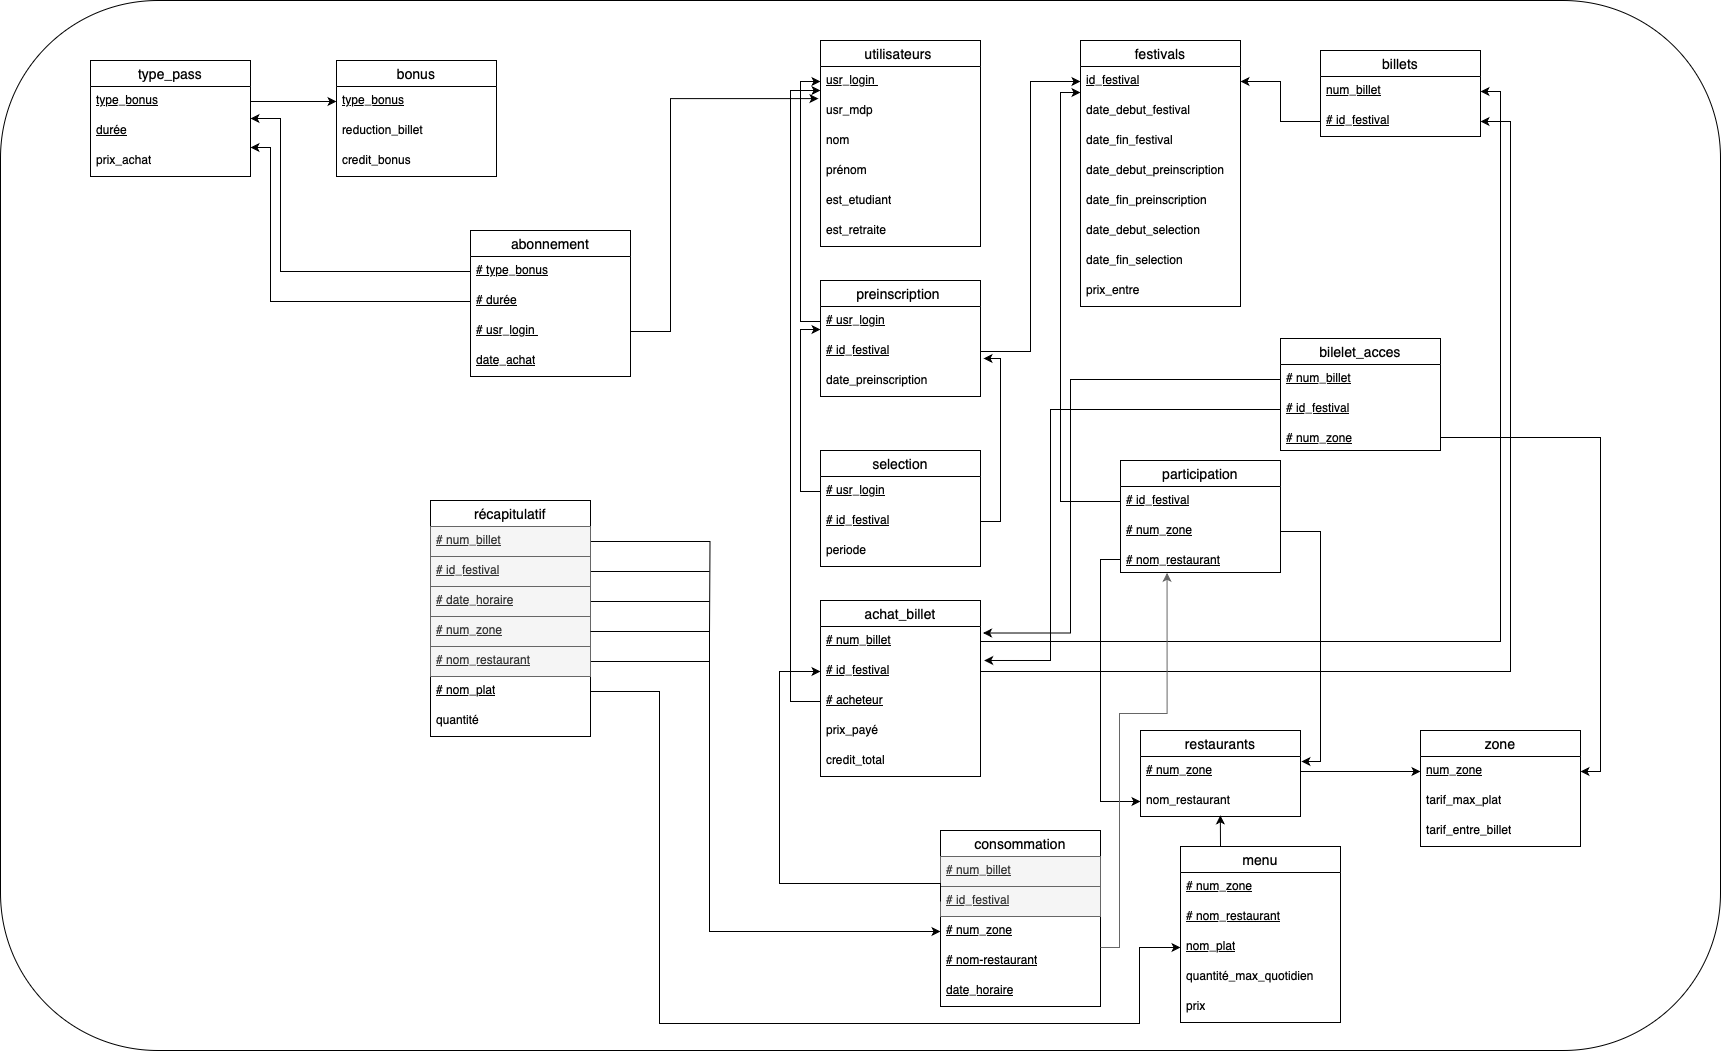
\includegraphics[width=1\textwidth]{schema_relationnel.png}
    \caption{Schema relationnel.}
    \label{fig:monimage}
\end{figure}

\section{Index}

Dans notre base de données, nous utilisons principalement des index primaires, 
car nos clés primaires couvenrt déjà une grand partie des attributs de nos tables.
Cela limite naturellement le besoin en index secondaire,
tout en garantissant de bonne performances sur la majorité de nos requêtes. 
Toutefois, afin d'optimiser certains cas d'usage spécifiques, 
nous avons ajouté un index secondaire ciblé pour améliorer l'efficacité de certaines recherches précices comme la recherche d'intervalle de prix.


\section{Transactions}
On retrouve plusieurs utilisations de transactions dans notre systeme comme pour l'achat du billet ou de la création du ticket de consommation. (voir les scénarios)
L'achat du billet utilise notamment un lock en lecture.
La gestion d'erreur lors de la création d'un ticket de consommation utilise le rollack.

\section{Scenarios}

Dans le dossier ../ETUDES vous retrouverez plusieurs fichier .sql qui contienne des scénarios pour notre base de données.

\subsection{creation\_festivals.sql}

Ce fichier SQL sert à simuler l'ajout d'un nouveau festival dans la base de données ainsi que l'ensemble du processus lié aux préinscriptions, sélections et achats de billets.

\subsection{creation\_consommation.sql}
Ce fichier SQL permet de tester la création de consommations pendant un festival, la gestion concurrente des achats de plats par les participants, ainsi que le calcul du chiffre d'affaires des restaurants et du festival.
Il vérifie également les règles métiers liées aux soldes et aux limitations de consommation.

\subsection{creation\_transaction.sql}
Ce fichier SQL sert a tester les transactions.
Celui-ci possède la meme base que creation\_festivals.sql avec un exemple d'achat de billet qui est une action pouvant etre critique a l'aide des commandes SQL begin,commit,rollback.
Les transactions sont mis en commentaire et doivent etre éxécuté a part dans 2 terminals après que le fichier soit exécuté.

\subsection{creation\_ticket\_recapitulatif.sql} 
Ce fichier SQL sert a montrer un exemple d'utilisation d'une 
transaction avec rollback pour la gestion des erreurs lors de la creation 
d'un ticket de consommation lors de l'ajout d'un plat dans la consommation.

(voir ./ETUDES/readme.md pour plus d'informations)


\end{document}
